\RequirePackage{plautopatch}
\documentclass[a4paper,papersize,uplatex,dvipdfmx,10pt]{jsarticle}

%package類
%%%%%%%%%%%%%%%%%%%%
\usepackage[utf8]{inputenc} % エンコーディングが UTF8 であることを明示する。
%文書内リンク
% OTF フォントを使えるようにし、複数のウェイトも使用可能にする。
% これがないと、Mac のヒラギノ環境で使われる角ゴが太すぎてみっともない。
%\usepackage[deluxe]{otf}

% OT1→T1に変更し、ウムラウトなどを PDF 出力で合成文字ではなくす
\usepackage[T1]{fontenc}

% uplatex の場合に必要な処理
\usepackage[prefernoncjk]{pxcjkcat} % アクセントつきラテン文字を欧文扱いにする

% Helvetica と Times を sf と rm のそれぞれで使う。
% default だとバランスが悪いので、日本語に合わせて文字の大きさを調整する。
\usepackage[scaled=1.05,helvratio=0.95]{newtxtext}

% 色
\usepackage[dvipdfmx]{color}

\usepackage[colorlinks=true,allcolors=blue]{hyperref}
%\usepackage{hyperref} % 紙に印刷するときは青文字リンクは消す。

\usepackage{pxjahyper}%文字化け防止

\usepackage{array,amsmath,amssymb,bm,cases}%数式でよく使うもの

\usepackage[dvipdfmx]{graphicx}%画像使用

\usepackage{url}

\usepackage{natbib}

\usepackage{ascmac}%itembox環境

\usepackage{enumerate}%enumerate環境

% bibliography を目次に追加
\usepackage[nottoc,notlot,notlof]{tocbibind}

%\usepackage{mathtools}%dcases環境

\usepackage[nooneline]{subfigure}
\subfiguretopcaptrue

%\usepackage{comment}

\allowdisplaybreaks[4]

\usepackage{listings,jvlisting} %日本語のコメントアウトをする場合jvlisting(もしくはjlisting)が必要
%ここからソースコードの表示に関する設定
\lstset{
  basicstyle={\ttfamily},
  identifierstyle={\small},
  commentstyle={\smallitshape},
  keywordstyle={\small\bfseries},
  ndkeywordstyle={\small},
  stringstyle={\small\ttfamily},
  frame={tb},
  breaklines=true,
  columns=[l]{fullflexible},
  numbers=left,
  xrightmargin=0zw,
  xleftmargin=3zw,
  numberstyle={\scriptsize},
  stepnumber=1,
  numbersep=1zw,
  lineskip=-0.5ex
}
%ここまでソースコードの表示に関する設定

%newcommand類
%%%%%%%%%%%%%%%%%%%%
\newcommand{\bs}{\symbol{92}} %backslash

\newcommand{\red}[1]{\textcolor{red}{#1}} %文字色赤

\newcommand{\blue}[1]{\textcolor{blue}{#1}} %文字色青

\newcommand{\green}[1]{\textcolor{green}{#1}} %文字色緑

\newcommand{\ured}[1]{\textcolor{red}{\underline{\textcolor{black}{#1}}}} %下線赤

\newcommand{\ugreen}[1]{\textcolor{green}{\underline{\textcolor{black}{#1}}}} %下線緑

\newcommand{\ublue}[1]{\textcolor{blue}{\underline{\textcolor{black}{#1}}}} %下線青
%%%%%%%%%%%%%%%%%%%%

\title{天文学特選F\,レポート}
\author{宇宙地球物理学科\,\,天文学コース\\B9SB2107\,\,松本尚輝}
\date{\today}

\begin{document}
\maketitle
\section{宇宙モデル}
\subsection{スケール因子}
密度パラメータが
\begin{enumerate}[(a)]
  \item $\Omega_{m,0}=0.3$、$\Omega_{\Lambda,0}=0.7$
  \item $\Omega_{m,0}=0.3$、$\Omega_{\Lambda,0}=0.0$
  \item $\Omega_{m,0}=1.0$、$\Omega_{\Lambda,0}=0.0$
\end{enumerate}
である場合の宇宙モデルについて、スケール因子$a(t)$と時間$t$の関係式を導き、それを図にプロットする(プロットの際は比較のため、現在時間を$t=0$ととる)。また、光度距離$d_{\mathrm{L}}$及び角径距離$d_{\mathrm{A}}$を赤方偏移$z$の関数としてプロットする。



\subsection{Ia型超新星と加速膨張}
Ia型超新星の観測から宇宙は現在、加速膨張しているものと考えられている。これは、

\section{宇宙再電離}
\subsection{銀河間ガス}
現在の銀河間ガスが電離していることは、遠方クェーサーなどの放射スペクトルから説明される。これらの放射は観測者の視線方向のガスに吸収されて観測される。例えば、dumped Ly$\alpha$は原始銀河の円盤による吸収を受けた際などに現れる減衰ウィングである。中性水素はライマン$\alpha$線を自由束縛遷移で吸収するので、銀河間ガスが中性であれば図~\ref{fig_lya}のように地球上($z=0$)で観測されるスペクトルに$121.6\,\mathrm{nm}$より長波長側で連続的な吸収を受けるはずである。

$z<6$のクェーサーに対してはそのような連続吸収が存在しない一方で、$z>6$ではこのような連続的な吸収スペクトルが見られるクェーサーが確認されている。このため$z\sim6$で銀河間ガスが電離する、\textbf{宇宙再電離}が起きたと考えられている。

\begin{figure}
	\centering
	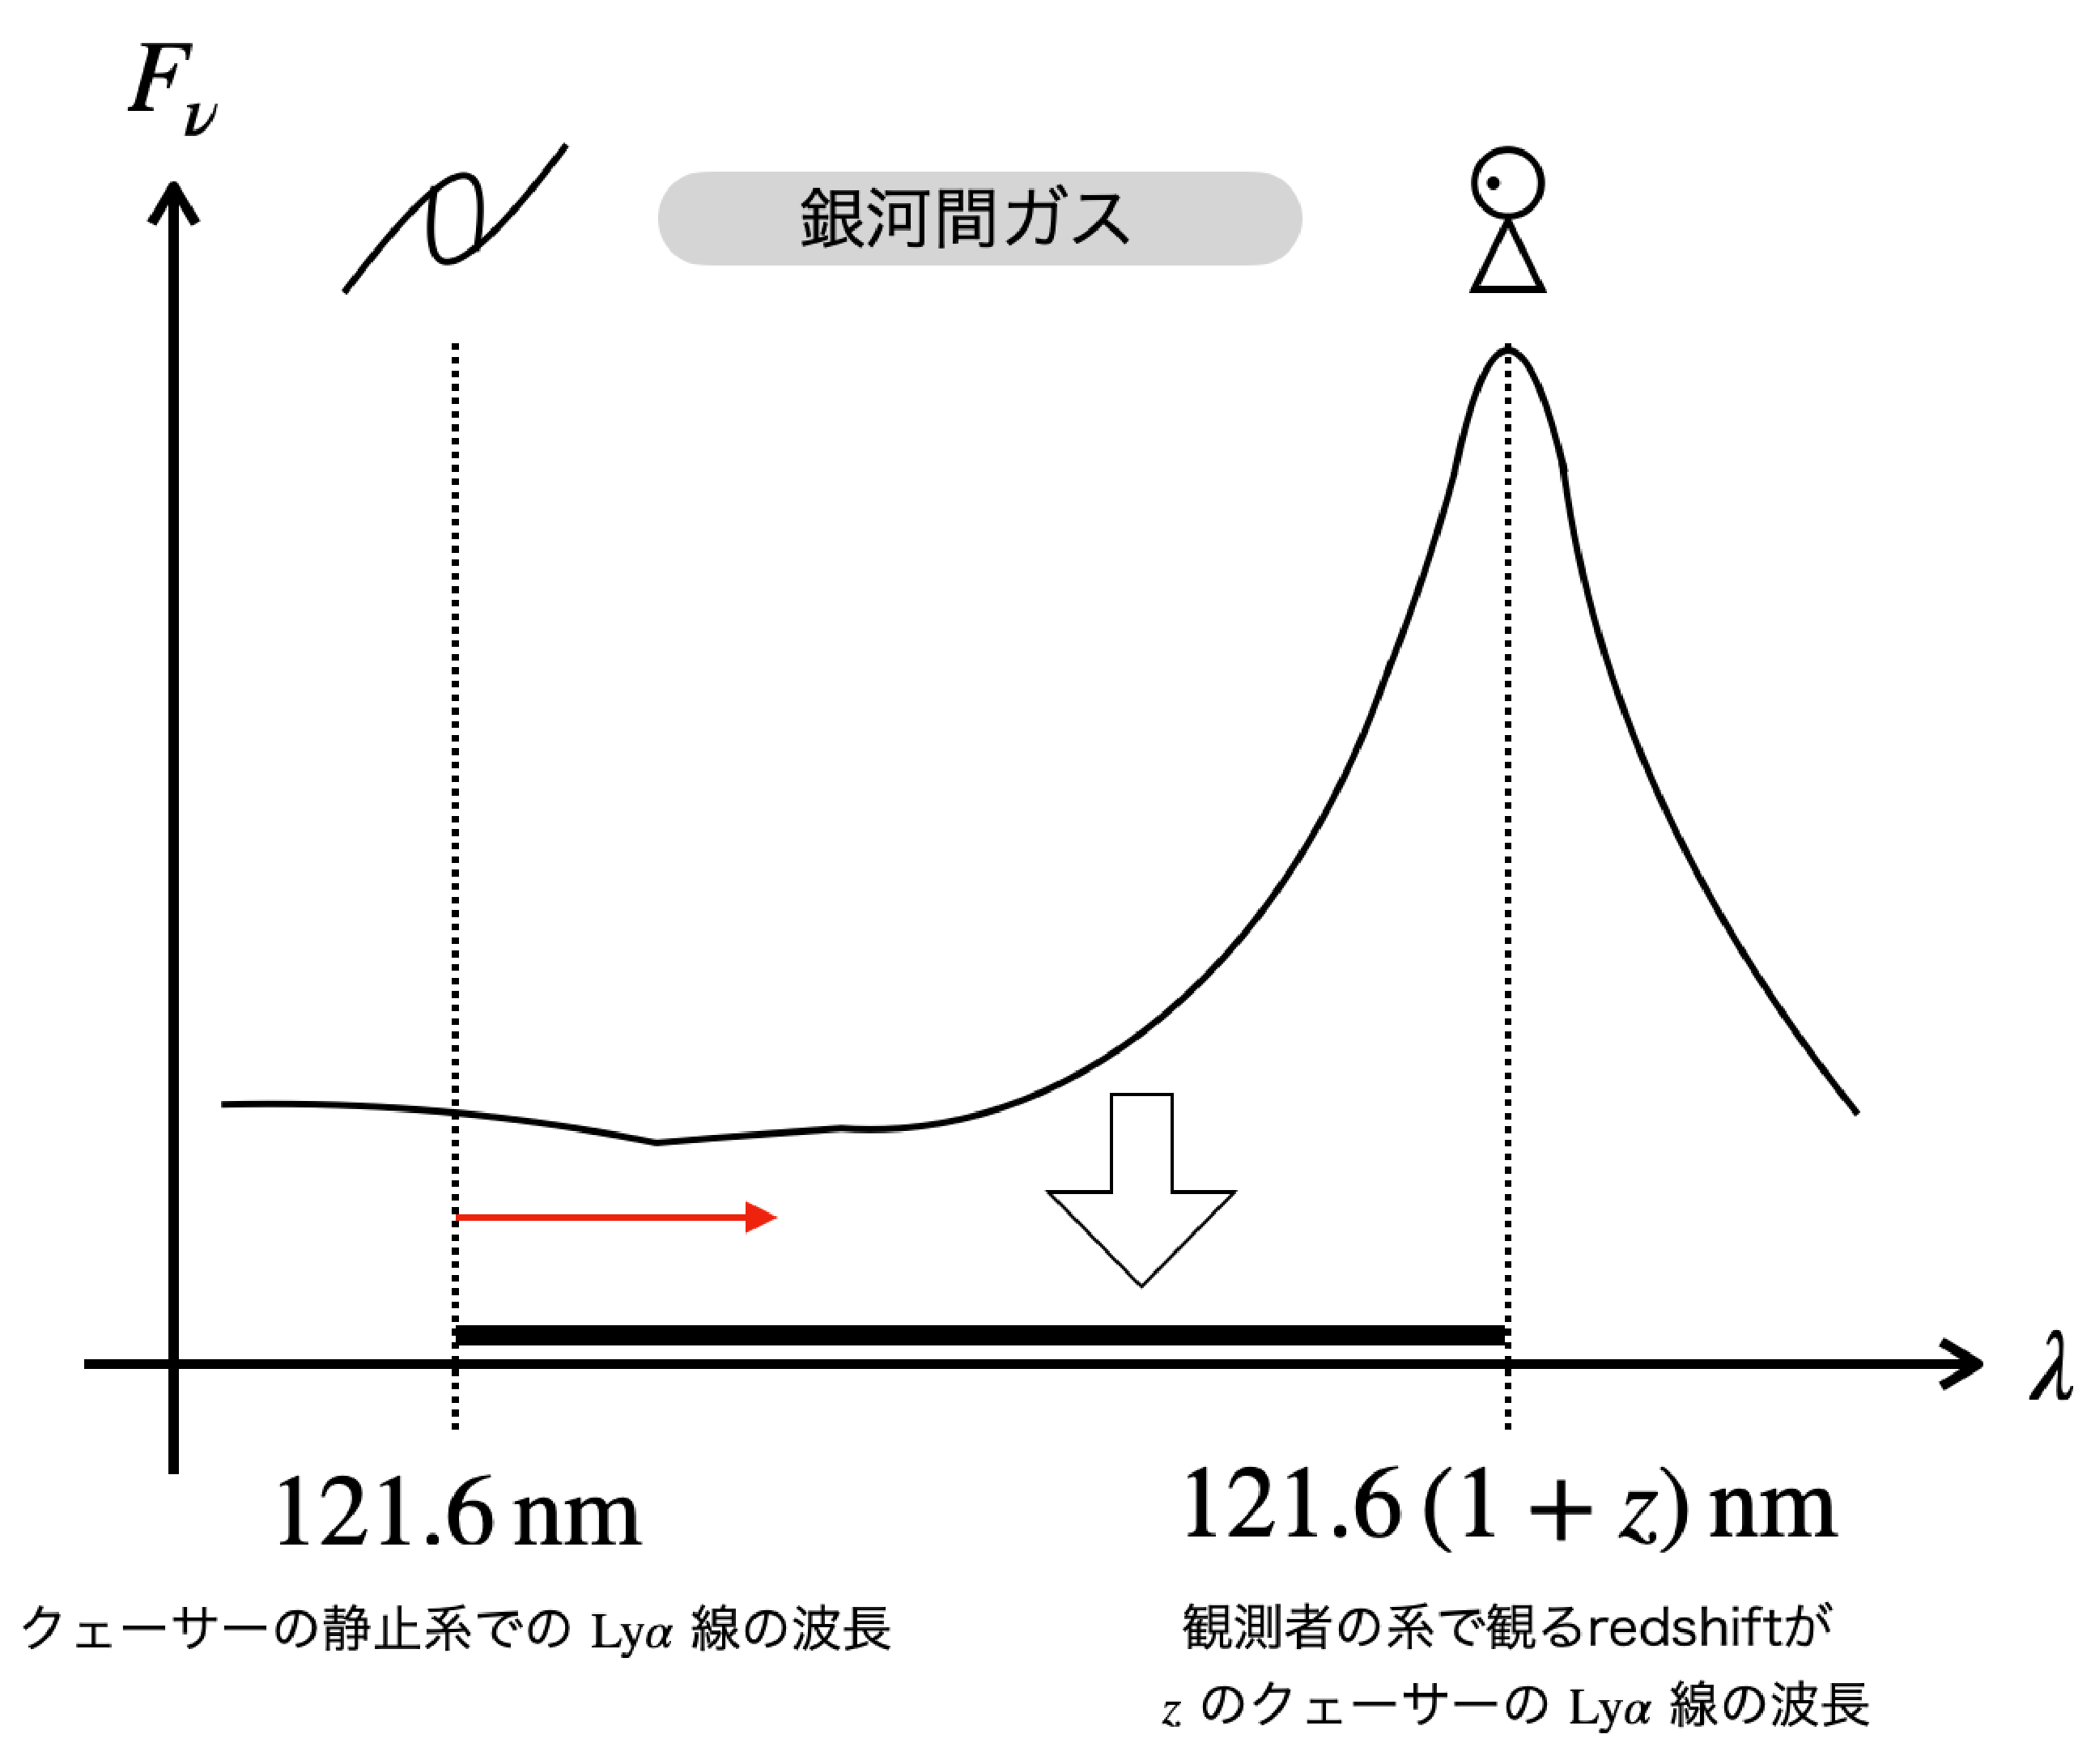
\includegraphics[width=0.6\linewidth]{fig/lyalpha.pdf}
	\caption{Ly$\alpha$線の銀河間ガスによる吸収 \label{fig_lya}}
\end{figure}

\subsection{トムソン散乱の光学的厚み}
再結合後、それまで中性だった銀河間ガスが、ある赤方偏移$z_{\mathrm{reion}}$で突然再電離したとして、銀河間ガスの数密度が$n=n_{0}(1+z)^{3}$としたときに、再電離によるトムソン散乱の光学的厚みが
\begin{align}
  \tau_{e} = \frac{2\mathrm{c}\sigma_{\mathrm{T}}n_{0}}{3\Omega_{m,0}H_{0}}\left( \left[ \Omega_{m,0}(1+z_{\mathrm{reion}})^{3}+\Omega_{\Lambda,0} \right]^{\frac{1}{2}}-1 \right)
\end{align}
と与えられることを示す。ただし、$\Omega_{m,0}+\Omega_{\Lambda,0}=1$の宇宙モデルを考え、$\sigma_{\mathrm{T}}$はトムソン散乱断面積である。

\subsection{CMBの偏光観測}
CMBの偏光観測から$\tau_{e}=0.06$程度と想定されているが、この時の$z_{\mathrm{reion}}$がどのような値となるか考える。

\section{密度ゆらぎの分散}
密度ゆらぎの$2$乗$\sigma^{2}(M)$が
\begin{align}
  \sigma^{2}(M) = \left< \left( \frac{\delta M}{M} \right)^{2} \right> = \int^{R^{-1}}_{0}\Delta^{2}(k)\,\mathrm{d}\ln{k}
\end{align}
となることを示す。ただし、
\begin{align}
  \Delta^{2}(k) = \frac{k^{3}}{2\pi^{2}}P(k)
\end{align}
で、$P(k)$は密度ゆらぎのパワースペクトルである。

\section{密度ゆらぎの進化}
物質優勢期の密度ゆらぎの進化について考える。
\subsection{共動座標系への変換}
自己重力流体の基礎方程式は
\begin{align}
  \text{(連続の式)}&:\frac{\partial \rho}{\partial t}+\bm{\nabla}\cdot\left( \rho \mathbf{v} \right)=0 \label{renzoku}\\
  \text{(Euler方程式)}&:\frac{\partial \mathbf{v}}{\partial t}+\mathbf{v}\cdot\nabla\mathbf{v}=-\nabla \phi \label{euler}\\
  \text{(Poisson方程式)}&:\nabla^{2}\phi = 4\pi\mathrm{G}\rho \label{poisson}
\end{align}
のように与えられる。

これを物理座標$(t,\mathbf{r})$から共動座標$(t^{\prime},\mathbf{x})$に変換する。ただし、
\begin{equation}
  \mathbf{r} = a(t)\mathbf{x}
\end{equation}
\begin{equation}
  \mathbf{v}=\dot{\mathbf{r}}=\dot{a}\mathbf{x}+a\dot{\mathbf{x}}=a\left( H\mathbf{x}+\mathbf{u} \right)
\end{equation}
\begin{equation}
  H \equiv \frac{\dot{a}}{a},\mspace{10mu}\mathbf{u}\equiv\dot{\mathbf{x}}
\end{equation}
であり、実効的な重力ポテンシャル$\Phi$を
\begin{equation}
  \Phi \equiv \left( \phi + \frac{1}{2}a\ddot{a}x^{2} \right)
\end{equation}
とし、物質優勢期におけるフリードマン方程式
\begin{align}
  \frac{\ddot{a}}{a} = -\frac{4\pi\mathrm{G}}{3}\bar{\rho},\mspace{20mu}(\rho=\bar{\rho}(1+\delta))
\end{align}
を用いる。

まず、座標変換に対して微分演算子がどのように変換されるかを確かめる。任意のスカラー量$Q$に対して、
\begin{align}
  \frac{\partial Q}{\partial t} &= \frac{\partial Q}{\partial t^{\prime}}\left.\frac{\partial t^{\prime}}{\partial t}\right|_{\mathbf{r}} + \frac{\partial Q}{\partial \mathbf{x}}\left.\frac{\partial \mathbf{x}}{\partial t}\right|_{\mathbf{r}}\notag\\
  &= \frac{\partial Q}{\partial t^{\prime}} - H\mathbf{x}\cdot\frac{\partial Q}{\partial \mathbf{x}}
\end{align}
となることから、
\begin{equation}
  \frac{\partial}{\partial t} \to \frac{\partial}{\partial t^{\prime}} - H\mathbf{x}\cdot\bm{\nabla}_{\mathbf{x}}
\end{equation}

ただし$t^{\prime}=t$と
\begin{align*}
  \left.\frac{\partial \mathbf{x}}{\partial t}\right|_{\mathbf{r}} = \frac{\partial}{\partial t}\left( \frac{\mathbf{r}}{a} \right) &= \frac{\mathrm{d}a}{\mathrm{d}t}\frac{\partial}{\partial a}\left( \frac{\mathbf{r}}{a} \right)\\
  &= \dot{a}\left( -\frac{\mathbf{r}}{a^{2}} \right) = -H\mathbf{x}
\end{align*}
を使った。

同様に
\begin{align}
  \bm{\nabla}_{\mathbf{r}}Q = \frac{\partial Q}{\partial \mathbf{r}} &= \frac{\partial Q}{\partial t^{\prime}}\left.\frac{\partial t^{\prime}}{\partial \mathbf{r}} \right|_{\mathbf{r}} + \frac{\partial Q}{\partial \mathbf{x}}\left.\frac{\partial \mathbf{x}}{\partial \mathbf{r}}\right|_{\mathbf{r}}\notag\\
  &= \frac{1}{a}\frac{\partial Q}{\partial \mathbf{x}}
\end{align}
となるので、
\begin{equation}
  \bm{\nabla}_{\mathbf{r}} \to \frac{1}{a}\bm{\nabla}_{\mathbf{x}}
\end{equation}

途中で
\begin{align*}
  \left.\frac{\partial t^{\prime}}{\partial \mathbf{r}} \right|_{\mathbf{r}} &= \frac{\partial t}{\partial \mathbf{r}} = 0\\
  \left.\frac{\partial \mathbf{x}}{\partial \mathbf{r}}\right|_{\mathbf{r}} &= \frac{\partial}{\partial \mathbf{r}}\left( \frac{\mathbf{r}}{a} \right) = \frac{1}{a}
\end{align*}
を用いた。

いま導出した式を使って式~\eqref{renzoku}、\eqref{euler}、\eqref{poisson}を変換する。
\subsubsection{連続の式}
\begin{align}
  \frac{\partial \rho}{\partial t} &\to \frac{\partial \rho}{\partial t^{\prime}} - \left( H\mathbf{x}\cdot\bm{\nabla}_{\mathbf{x}}\right)\rho\\
  \bm{\nabla}_{\mathbf{r}}\cdot\left( \rho \mathbf{v} \right) &\to \frac{1}{a}\bm{\nabla}_{\mathbf{x}}\cdot\left( \rho aH\mathbf{x} + \rho a\mathbf{u} \right)\notag\\
  &= 3H\rho + \left( H\mathbf{x}\cdot\bm{\nabla}_{\mathbf{x}}\right)\rho + \bm{\nabla}_{\mathbf{x}} \cdot \left( \rho\mathbf{u} \right)
\end{align}
よって、
\begin{equation}
  \text{(連続の式)}: \frac{\partial \rho}{\partial t} + 3H\rho + \bm{\nabla}_{\mathbf{x}} \cdot \left( \rho\mathbf{u} \right) = 0
\end{equation}

\subsubsection{Euler方程式}
\begin{align}
  \frac{\partial \mathbf{v}}{\partial t} &\to \frac{\partial}{\partial t^{\prime}}\left( a\left( H\mathbf{x}+\mathbf{u} \right) \right) - \left( H\mathbf{x}\cdot\bm{\nabla}_{\mathbf{x}} \right)\left\{ a\left( H\mathbf{x}+\mathbf{u} \right) \right\}\\
  \left( \mathbf{v}\cdot\bm{\nabla}_{\mathbf{r}} \right)\mathbf{v} &\to \left\{ \left( H\mathbf{x}+\mathbf{u} \right)\cdot\bm{\nabla}_{\mathbf{x}} \right\}\left( a\left( H\mathbf{x}+\mathbf{u} \right) \right)\notag\\
  &=\left( H\mathbf{x}\cdot\bm{\nabla}_{\mathbf{x}} \right)\left\{ a\left( H\mathbf{x}+\mathbf{u} \right) \right\} + \left( \mathbf{u}\cdot\bm{\nabla}_{\mathbf{x}} \right)\left( aH\mathbf{x} \right) + \left( \mathbf{u}\cdot\bm{\nabla}_{\mathbf{x}} \right)a\mathbf{u}\\
  \nabla_{\mathbf{r}}\phi &\to \frac{1}{a}\bm{\nabla}_{\mathbf{x}}\left( \Phi - \frac{1}{2}a\ddot{a}x^{2} \right)
\end{align}
まとめると、
\begin{align*}
  \frac{\partial}{\partial t^{\prime}}\left( a\left( H\mathbf{x}+\mathbf{u} \right) \right) + \left( \mathbf{u}\cdot\bm{\nabla}_{\mathbf{x}} \right)\left( aH\mathbf{x} \right) + \left( \mathbf{u}\cdot\bm{\nabla}_{\mathbf{x}} \right)(a\mathbf{u}) = -\frac{1}{a}\bm{\nabla}_{\mathbf{x}}\left( \Phi - \frac{1}{2}a\ddot{a}x^{2} \right)
\end{align*}
$H=\dot{a}/a$、$\partial \mathbf{x}/\partial t^{\prime}=0$を用いて、
\begin{align*}
  \text{(左辺)}: &\left(\ddot{a}\mathbf{x}+\dot{a}\mathbf{u}+a\frac{\partial \mathbf{u}}{\partial t^{\prime}}\right)+\dot{a}\left(\mathbf{u}\cdot\bm{\nabla}_{\mathbf{x}}\right)\mathbf{x}+a\left(\mathbf{u}\cdot\bm{\nabla}_{\mathbf{x}}\right)\mathbf{u}\\
  &= \ddot{a}\mathbf{x} + \dot{a}\mathbf{u} + a\frac{\partial \mathbf{u}}{\partial t^{\prime}} + \dot{a}\mathbf{u} + a\left( \mathbf{u}\cdot\bm{\nabla}_{\mathbf{x}} \right)\mathbf{u}\\
  \text{(右辺)}: &-\frac{1}{a}\nabla_{\mathbf{x}}\Phi + \frac{1}{2}\ddot{a}\nabla_{\mathbf{x}}x^{2}\\
  &= -\frac{1}{a}\nabla_{\mathbf{x}}\Phi + \ddot{a}\mathbf{x}
\end{align*}



\subsection{ゆらぎの進化方程式}
密度ゆらぎの進化方程式
\begin{equation}
  \frac{\partial^{2} \delta}{\partial t^{2}}+2H\frac{\partial \delta}{\partial t}-4\pi\mathrm{G}\bar{\rho}\delta=0
\end{equation}
を導出する。

\subsection{Harrison-Zel'dovich spectrum}
宇宙の極初期に存在した原始密度揺らぎがHarrison-Zel’dovichスペクトル$P(k) \propto k$で与えられるとき、 等密度時以後の揺らぎスペクトルがどのようになるかを考える。

\section{初代星・初代銀河と巨大ブラックホール}
\subsection{初代星と初代銀河の形成}

\subsection{巨大ブラックホールの形成}


%\renewcommand{\bibname}{参考文献}
%\bibliographystyle{jecon}
%\bibliography{thesis}
\end{document}
